\documentclass[conference]{IEEEtran}
\IEEEoverridecommandlockouts
% IEEE requires Times. The classic \usepackage{times} sets Times New Roman for
% the text (and the matching math), is what the official IEEE templates use,
% and — unlike newtxmath — does not clash with amssymb. This is the explicit
% fix for the "Latin Modern default" font issue.
\usepackage{times}
\usepackage{cite}
\usepackage{amsmath,amssymb,amsfonts}
\usepackage{graphicx}
\usepackage{textcomp}
\usepackage{xcolor}
\usepackage[hyphens]{url}
\def\BibTeX{{\rm B\kern-.05em{\sc i\kern-.025em b}\kern-.08em T\kern-.1667em\lower.7ex\hbox{E}\kern-.125emX}}
\begin{document}

\title{A Multi-Protocol Cyber-Deception Framework Combining Language-Model Response Synthesis with Blockchain-Anchored Forensic Logging}

\author{
\IEEEauthorblockN{Radhika G\textsuperscript{1}, Sisir Reddy Nellore\textsuperscript{2}, Pranav Sharma Chouduru\textsuperscript{3}, Surya Tejeswar Reddy Nagireddy\textsuperscript{4},\\ Guru Sai Prasad Reddy Bompalli\textsuperscript{5}, Vishnu Sathwick Rajala\textsuperscript{6}}
\IEEEauthorblockA{\textit{Department of Computer Science and Engineering}\\
\textit{Amrita School of Computing, Coimbatore}\\
\textit{Amrita Vishwa Vidyapeetham, India}\\
g\_radhika@cb.amrita.edu\textsuperscript{1}, cb.sc.u4cse23129@cb.students.amrita.edu\textsuperscript{2},\\
cb.sc.u4cse23611@cb.students.amrita.edu\textsuperscript{3}, cb.sc.u4cse23127@cb.students.amrita.edu\textsuperscript{4},\\
cb.sc.u4cse23111@cb.students.amrita.edu\textsuperscript{5}, cb.sc.u4cse23644@cb.students.amrita.edu\textsuperscript{6}}
}

\maketitle

\begin{abstract}
Low- and medium-interaction honeypots remain a cost-effective source of attacker telemetry, but their reliance on fixed response tables makes them straightforward to fingerprint: a scanner that sends a handful of atypical requests can observe that the replies are drawn from a finite, deterministic set and disengage. We present a multi-protocol deception framework that replaces the fixed response table with a language-model (LM) response engine serving five heterogeneous decoys --- an interactive SSH shell, a PostgreSQL query endpoint, an internal AI/chat API, an Ethereum JSON-RPC node, and a Jenkins continuous-integration server --- behind a single connection-logging proxy. A three-tier response path answers routine traffic from a static fast-path and a cache in sub-millisecond time, and escalates only novel requests to the LM, preserving both realism and throughput. Every interaction is intent-classified by a transparent rule set, hashed with SHA-256, and anchored as a transaction on a local Ethereum chain, yielding a tamper-evident audit trail whose integrity does not depend on the logging host. We evaluate the system against a static-response baseline along four axes --- sequential latency and throughput, throughput under concurrent sessions, per-service response diversity, and an LM-judge realism score --- using a corpus of 2,500 real, publicly documented attack payloads spanning all five services. The dynamic path answers with a mean latency of 2.33 s against sub-millisecond static-path latency, sustains 1.61 requests/s under 10 concurrent sessions, and produces high output diversity for all five services (uniqueness ratio 0.64--0.992) versus the near-zero diversity of a static table by construction. The mean LM-judge realism score is 4.37/5; the small number of low-rated responses falls mostly on the AI-API decoy, which is the weakest service on both diversity and judged realism, and we report that per-service disparity rather than the favourable aggregate alone. We also document, as part of the contribution, the engineering gaps we identified and resolved during construction --- a latency optimisation, a benchmark-harness correction, and an intent-classifier that initially left most traffic unlabelled --- and the concrete limitations of an automated realism proxy as a substitute for a human-subject detectability study.
\end{abstract}

\begin{IEEEkeywords}
honeypot, cyber deception, large language models, blockchain, digital forensics, intrusion detection.
\end{IEEEkeywords}

\section{Introduction}

A honeypot is a decoy system deployed with no legitimate purpose, so that any interaction with it is, by definition, suspicious. Because they generate high-signal telemetry at low operational risk, honeypots are a standard component of threat-intelligence and early-warning pipelines. The dominant low- and medium-interaction designs --- exemplified by SSH/Telnet decoys that emulate a shell without booting a real operating system --- achieve their low cost precisely by not being real: they answer from a hand-written table of canned responses. This is also their central weakness. An automated scanner that issues even a few commands outside the table observes responses that are missing, inconsistent, or identical across supposedly distinct hosts, and concludes it is talking to a decoy. Vetterl and Clayton [5] showed that such fingerprinting can be performed at Internet scale with a single packet, at an equal-error rate of 0.0183, identifying 2,844 real Cowrie and Kippo honeypot instances in the wild.

The problem is structural, not a matter of writing a larger table. Any finite, static response set is enumerable, and an adversary who enumerates it can distinguish the decoy from a genuine service. What is needed is a response mechanism that is \emph{generative} rather than \emph{tabular} --- one that can produce a plausible, context-consistent reply to a request never seen before.

Modern language models are a natural fit for this role. An instruction-tuned model, prompted to emulate the raw output stream of a specific service, can synthesise responses to arbitrary inputs while maintaining session consistency. This capability, however, introduces two engineering tensions that a deployable system must resolve. First, an LM call costs on the order of seconds, whereas a real service answers routine requests in microseconds; a naïve "every request goes to the model" design is both slow and expensive, and its latency profile is itself a fingerprinting signal. Second, an LM occasionally breaks character --- emitting a refusal, a disclaimer, or an explanatory aside that no real service would produce --- which is a deception-fatal tell rather than a minor stylistic flaw.

A second, orthogonal concern is the integrity of the collected evidence. A honeypot log that is only a file on the collecting host is only as trustworthy as that host. If the honeypot is compromised --- a real risk, since its entire purpose is to be attacked --- the attacker can edit or delete the very records of the intrusion. For telemetry that is to be used as forensic evidence, the audit trail needs an integrity guarantee that survives compromise of the logging system itself.

This paper describes a framework that addresses both concerns together and reports an honest evaluation of the result. Our contributions are:

\begin{enumerate}
\item \textbf{A multi-protocol, LM-backed deception layer} covering five distinct modern attack surfaces (SSH, SQL, an internal AI API, an Ethereum RPC node, and a CI/CD server) behind one logging proxy, with a three-tier response path that keeps routine traffic fast while reserving generative responses for novel inputs.
\item \textbf{Blockchain-anchored forensic logging}, in which every interaction is hashed and the hash is committed on-chain, giving each record tamper-evidence independent of the honeypot host, verifiable after the fact by any party.
\item \textbf{A four-axis evaluation against a static baseline} on a corpus of real, publicly documented attack payloads --- measuring latency/throughput, concurrent throughput, per-service response diversity, and an LM-judge realism score --- that reports the system's failure modes (a specific decoy whose realism is poor, and the limits of automated realism scoring) as explicitly as its successes.
\end{enumerate}

The remainder of the paper is organised as follows. Section 2 reviews related work. Section 3 states the threat model and design goals. Section 4 describes the architecture, Section 5 the evaluation method, and Section 6 the results. Section 7 documents the engineering gaps we identified and resolved during construction and measurement, and Section 8 compares the framework with prior systems. Section 9 discusses trade-offs and threats to validity, Section 10 the limitations and future work, and Section 11 concludes.

\section{Related Work}

We organise prior work into four strands --- classical honeypots and their detectability, LLM-backed deception, secure and blockchain-anchored logging, and the broader deception/evaluation literature --- and position our contribution against each.

\subsection{Classical honeypots and fingerprinting}

Honeypots have been a standard sensor since Spitzner's foundational treatment [1] and Provos's Honeyd virtual-honeypot framework [2]. The widely deployed low- and medium-interaction systems --- the Cowrie SSH/Telnet honeypot [3] and the malware-capturing Dionaea [4] --- emulate services from fixed response logic, which makes them cheap and safe but also enumerable. Vetterl and Clayton [5] made this concrete at scale: exploiting the fact that such honeypots reuse off-the-shelf protocol libraries whose behaviour deviates subtly from the real service, they fingerprinted low/medium-interaction honeypots with a single packet at an equal-error rate of 0.0183, locating 2,844 real Cowrie and Kippo instances on the Internet. This structural weakness --- a finite, deterministic response set is always distinguishable from a real service --- is the core problem a generative response mechanism is meant to solve.

\subsection{LLM-backed generative honeypots}

Replacing the fixed table with a language model was proposed conceptually by McKee and Noever [10], who showed ChatGPT imitating Linux, Mac, and Windows terminal commands. Sladić et al.'s ShelLM [11] was the first integrated generative SSH honeypot and remains the strongest published realism result: in a human-subject study of 226 commands it reached 0.92 accuracy and a 0.90 true-negative rate. Subsequent systems refined the architecture: HoneyGPT [12] added a dedicated prompt-management component to track session state and framed its design as resolving a three-way tension between flexibility, depth of interaction, and deception quality; HoneyLLM [13] added a filter/router front end and reported a mean 1.88 s per command against a 0.138 s Cowrie baseline. A recent systematisation by Bridges et al. [15] catalogues sixteen such systems and distils a canonical architecture --- filter/router, deterministic (cached) responder, prompt and state manager, and LLM engine --- that our tiered design independently mirrors. Two limitations recur across this literature and directly motivate our work. First, realism is fragile: Weber et al. [14] found in a human study that only 52\% of GPT-3.5 honeypot responses were convincing, with compound commands the main failure mode --- a caution we echo in our own AI-API result. Second, and more fundamentally for our contribution, every system in this line targets a \emph{single} surface (a Linux shell) and none anchors its logs for integrity. We extend the generative approach to five heterogeneous protocols and add tamper-evident logging, while engaging the same three open problems the literature identifies --- latency/cost, session consistency, and character stability.

\subsection{Secure and blockchain-anchored logging}

The integrity of security logs is a long-studied problem. Schneier and Kelsey [17] introduced secure audit logs resistant to tampering by an attacker who compromises the logging host, and Ma and Tsudik [18] advanced forward-secure sequential aggregate authentication for the same threat. More recently, distributed ledgers have been used to anchor log integrity: instead of placing the full data on-chain, only a short hash of each record is written to the ledger, so that any subsequent edit is caught by recomputing the hash and comparing it against the committed value, as in Sutton and Samavi's blockchain-enabled audit logs [21], building on the integrity guarantees of the Bitcoin [19] and Ethereum [20] ledgers. We apply this well-established pattern specifically to honeypot telemetry --- a setting where the logging host is, by design, the thing being attacked --- so that the evidentiary value of the logs does not rest on the integrity of the collecting host. To our knowledge this coupling of a generative multi-protocol honeypot with on-chain log anchoring has not previously been reported.

\subsection{Deception frameworks, honeytokens, and evaluation}

Beyond service emulation, a broad literature places decoys throughout an environment: Han et al.'s survey of deception techniques [6] frames the design space, Bowen et al. [7] embed beacons in decoy documents to bait insiders, and Juels and Rivest's honeywords [8] plant decoy passwords to detect credential theft; recent surveys track the field's evolution toward honeypot performance [9]. Our contribution is complementary and narrower: a self-contained multi-protocol decoy cluster with a generative response layer and integrity-anchored logging. On evaluation, human-subject detectability studies remain the gold standard [11], [14] but are costly; automated proxies --- output diversity and, increasingly, using a second model as a judge (the LLM-as-judge paradigm [22]) --- are cheaper but imperfect. We adopt both diversity and an LM judge and are explicit (Section 5.3) that the judge is a proxy, reporting where it is unreliable rather than treating its score as ground truth. Automated downstream analysis of the resulting telemetry --- e.g. mapping captured commands to MITRE ATT\&CK [23] tactics, as LogPrécis [16] does at over 90\% accuracy --- is a natural consumer of the intent-classified, integrity-anchored logs our framework produces.

\section{Threat Model and Design Goals}

\subsection{Adversary model}

We consider two adversary classes, following the distinction the recent literature draws [15]. The first is the \emph{automated scanner}: a high-rate, non-interactive bot that probes exposed services, issues a small set of stereotyped requests, and moves on. Such scanners dominate real honeypot traffic --- field studies report that the overwhelming majority of honeypot activity is automated scanning rather than hands-on-keyboard interaction [15] --- and they fingerprint by looking for deterministic, enumerable, or internally-inconsistent responses [5]. The second is the \emph{interactive intruder}: a human (or human-directed agent) who has reached a shell or service and explores it at human speed, issuing novel, context-dependent commands. The two classes stress different properties --- the scanner stresses breadth, consistency, and latency uniformity; the intruder stresses the ability to answer genuinely novel input in character.

We further assume the honeypot host itself may be compromised: its entire purpose is to be attacked, so an adversary who gains sufficient access could attempt to alter or delete the very records of the intrusion. The integrity mechanism must therefore not rely on trusting the collecting host. We treat the blockchain node as an append-only integrity anchor and assume standard cryptographic hardness of SHA-256 and of the underlying ledger; we do not claim confidentiality of the logged data, only tamper-evidence.

\subsection{Design goals}

From this model we derive the requirements the rest of the paper is built and evaluated against:

\begin{itemize}
\item \textbf{G1 --- Non-enumerable responses.} Output must not collapse to a small deterministic set an automated probe can cluster (addresses the scanner; evaluated as response diversity, Section 6.3).
\item \textbf{G2 --- Novel-input handling.} The system must answer requests never seen before with plausible, context-consistent output (addresses the intruder; evaluated as realism, Section 6.4).
\item \textbf{G3 --- Latency compatible with a real service.} Routine traffic must be answered fast enough that timing is not itself a tell (Section 6.1).
\item \textbf{G4 --- Multi-protocol coverage.} A single framework should span several distinct modern attack surfaces rather than one (Section 4.2).
\item \textbf{G5 --- Host-independent log integrity.} Every record must be verifiable as untampered even if the honeypot host is compromised (Section 6.5).
\item \textbf{G6 --- Actionable, auditable classification.} Captured interactions should be labelled by attack intent using an explainable mechanism suitable for forensic use (Section 4.4).
\end{itemize}

Sections 4--6 map each goal to a mechanism and a measurement; Section 9 revisits where the goals are met and where they are only partially met.

\section{System Architecture}

The framework is a set of containerised services on an isolated bridge network. Only two components are reachable from outside: the connection proxy (which fronts the decoys) and the monitoring dashboard. The decoys, the response engine, the datastore, and the blockchain node communicate only on the internal network, so an attacker interacting with a decoy cannot reach the control plane directly. Fig. 1 shows the component layout and the trust boundary between the public interface and the internal network; Fig. 2 traces the sequence of a single interaction from connection through anchoring and live display.

\begin{figure*}[!t]
\centering
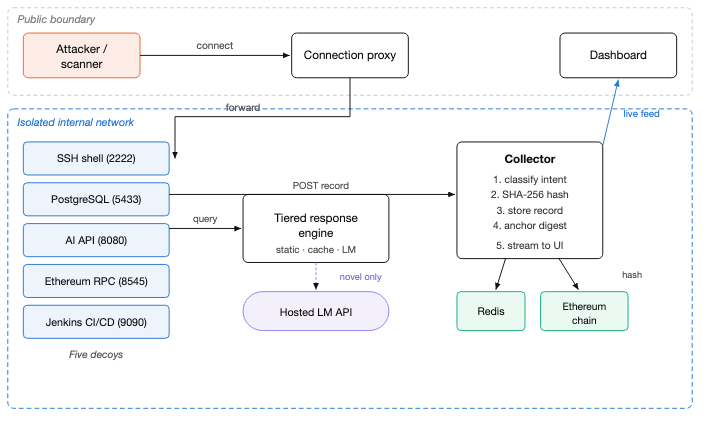
\includegraphics[width=\textwidth]{figures/diag_arch.png}
\caption{System architecture. Only the proxy and dashboard are on the public boundary; the five decoys, response engine, collector, datastore, and blockchain node communicate solely on the isolated internal network.}
\label{fig:arch}
\end{figure*}

\begin{figure*}[!t]
\centering
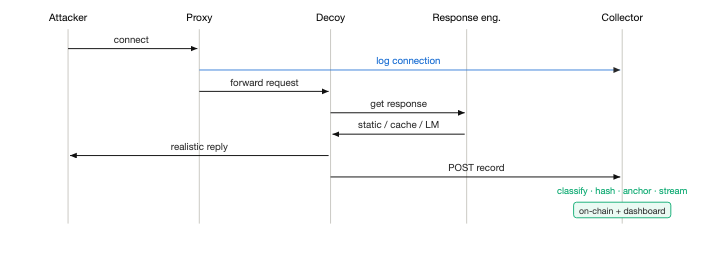
\includegraphics[width=\textwidth]{figures/diag_flow.png}
\caption{Data flow for one interaction: the proxy logs the connection before any decoy responds; the collector classifies, hashes, anchors on-chain, and streams to the dashboard.}
\label{fig:flow}
\end{figure*}

\subsection{Connection proxy and network isolation}

A single asynchronous proxy listens on the five public decoy ports and transparently forwards each connection to the corresponding internal decoy. It records every inbound connection --- source address and target port --- before any decoy responds, so that even a bare port scan that never completes a protocol handshake is captured. Separating the public-listening concern from the decoy logic keeps the decoys off the public interface and gives a single choke point for connection-level telemetry.

\subsection{Decoy services}

Five decoys cover distinct, currently relevant attack surfaces:

\begin{itemize}
\item \textbf{SSH shell (port 2222)} --- a real SSH server that accepts any credentials and presents an interactive shell identifying itself as a corporate Ubuntu database host. Login attempts and every subsequent command are logged; command output is produced by the tiered response path (Sec.~3.3).
\item \textbf{PostgreSQL endpoint (port 5433)} --- accepts SQL queries and returns plausible tabular results or realistic error text, baiting SQL-injection.
\item \textbf{Internal AI API (port 8080)} --- an "internal" chat/prediction service, a target for prompt-injection and jailbreak attempts.
\item \textbf{Ethereum JSON-RPC node (port 8545)} --- responds to the JSON-RPC methods that attackers invoke against exposed nodes to enumerate and drain wallets.
\item \textbf{Jenkins CI/CD server (port 9090)} --- exposes build- and script-oriented endpoints that represent the documented Jenkins attack surface.
\end{itemize}

Each decoy forwards a normalised record of every interaction to the central collector.

\subsection{Three-tier response path}

Generating every response with the LM would be slow, costly, and --- because of the uniform multi-second latency --- itself detectable. The response engine therefore uses three tiers, escalating only when necessary:

\begin{enumerate}
\item \textbf{Static fast-path.} The most common enumeration commands (for example directory listing, identity, and network-configuration queries on the SSH decoy) are answered from a fixed table in sub-millisecond time. This intercepts the bulk of routine traffic without an LM call. The realism cost is low, because these commands genuinely have stable, well-known outputs on a real host.
\item \textbf{Response cache.} Previously seen requests (keyed on the request and recent session context) are served from an in-memory cache, so a repeated probe does not incur a second LM call.
\item \textbf{Language-model synthesis.} Only novel requests reach the LM, which is prompted with a service-specific system persona instructing it to emit solely the raw output stream of the emulated service --- no explanation, no markdown, no acknowledgement that it is a model --- together with recent session history for consistency. The model used in our deployment is an instruction-tuned Llama-3.1-8B served through a hosted inference API, so the framework requires no local GPU.
\end{enumerate}

This structure bounds the \emph{expected} per-request cost: the fast-path and cache absorb routine load at near-zero latency, and only the genuinely novel tail pays the LM latency. Fig. 3 shows the decision path and the latency branch each tier returns on.

\begin{figure}[!t]
\centering
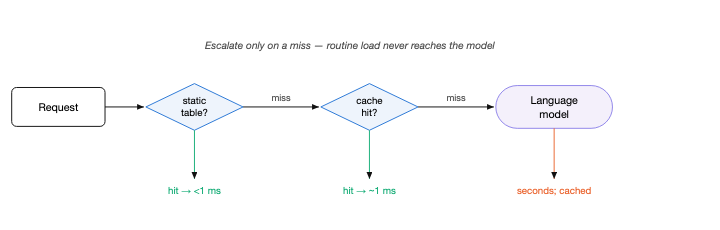
\includegraphics[width=\columnwidth]{figures/diag_tier.png}
\caption{Three-tier response path. Routine requests are answered from the static table or cache in sub-millisecond time; only novel requests reach the language model.}
\label{fig:tier}
\end{figure}

\subsection{Intent classification}

Every interaction is labelled with an attack-intent category by a transparent, rule-based classifier operating on the raw request text. The categories are \emph{SQL injection}, \emph{prompt injection}, \emph{crypto theft} (abusive Ethereum RPC methods such as wallet unlock/transfer), \emph{cryptomining}, \emph{reverse shell / RCE}, \emph{privilege escalation} (including brute-force login attempts and credential/ secret access), \emph{supply-chain / CI-CD abuse}, and \emph{reconnaissance} (scanning, service enumeration, and the standard first-contact commands on a fresh shell); anything unmatched is labelled \emph{unknown}. The classifier is intentionally rule-based rather than learned: the rules are auditable, need no training data, add no latency, and their decisions are explainable --- properties we consider more valuable for a forensic sensor than the marginal coverage a learned model might add. We stress that the language model performs response \emph{synthesis}, not classification; classification is a separate, deterministic stage.

\subsection{Blockchain-anchored logging}

When a record reaches the collector it is (i) intent-classified, (ii) serialised deterministically and hashed with SHA-256, and (iii) anchored by sending a transaction carrying that hash to a local Ethereum chain. The full record is retained in the datastore; only the digest is placed on-chain. The integrity guarantee follows directly: to check a record later, one re-hashes it and compares against the value committed on-chain. Any post-hoc alteration of the stored record --- by an attacker who has compromised the honeypot, or by anyone else --- changes its hash and is therefore detectable, because the on-chain digest cannot be silently rewritten. Integrity thus does not depend on trusting the logging host. Fig. 4 depicts both the anchoring step and the later verification that detects tampering.

\begin{figure}[!t]
\centering
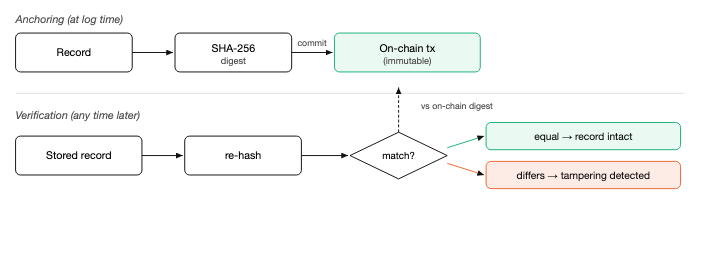
\includegraphics[width=\columnwidth]{figures/diag_chain.png}
\caption{Anchoring and tamper verification. A record's SHA-256 digest is committed on-chain; re-hashing and comparison later detects any modification.}
\label{fig:chain}
\end{figure}

\subsection{Real-time dashboard}

A web dashboard consumes the collector's live event stream and aggregate statistics. It presents intercepted-attack counts, per-intent and per-service breakdowns, ranked source addresses with a per-actor threat profile, and a searchable live feed in which each event exposes its payload, the decoy's response, its SHA-256 digest, and its on-chain anchoring status. The dashboard is the operator's view of the sensor and the surface used for the live integrity demonstration in Sec.~6. Fig. 5 is a live capture of the dashboard during operation, showing the intent breakdown, per-service exposure, and anchoring status over 6{,}742 intercepted events. Fig. 11 shows the per-attacker drill-down: for each source address the dashboard reconstructs the services it touched, a severity-weighted threat rating, its intent mix, and a timeline of the actual payloads it sent --- every entry marked with its on-chain anchoring status.

\begin{figure*}[!t]
\centering
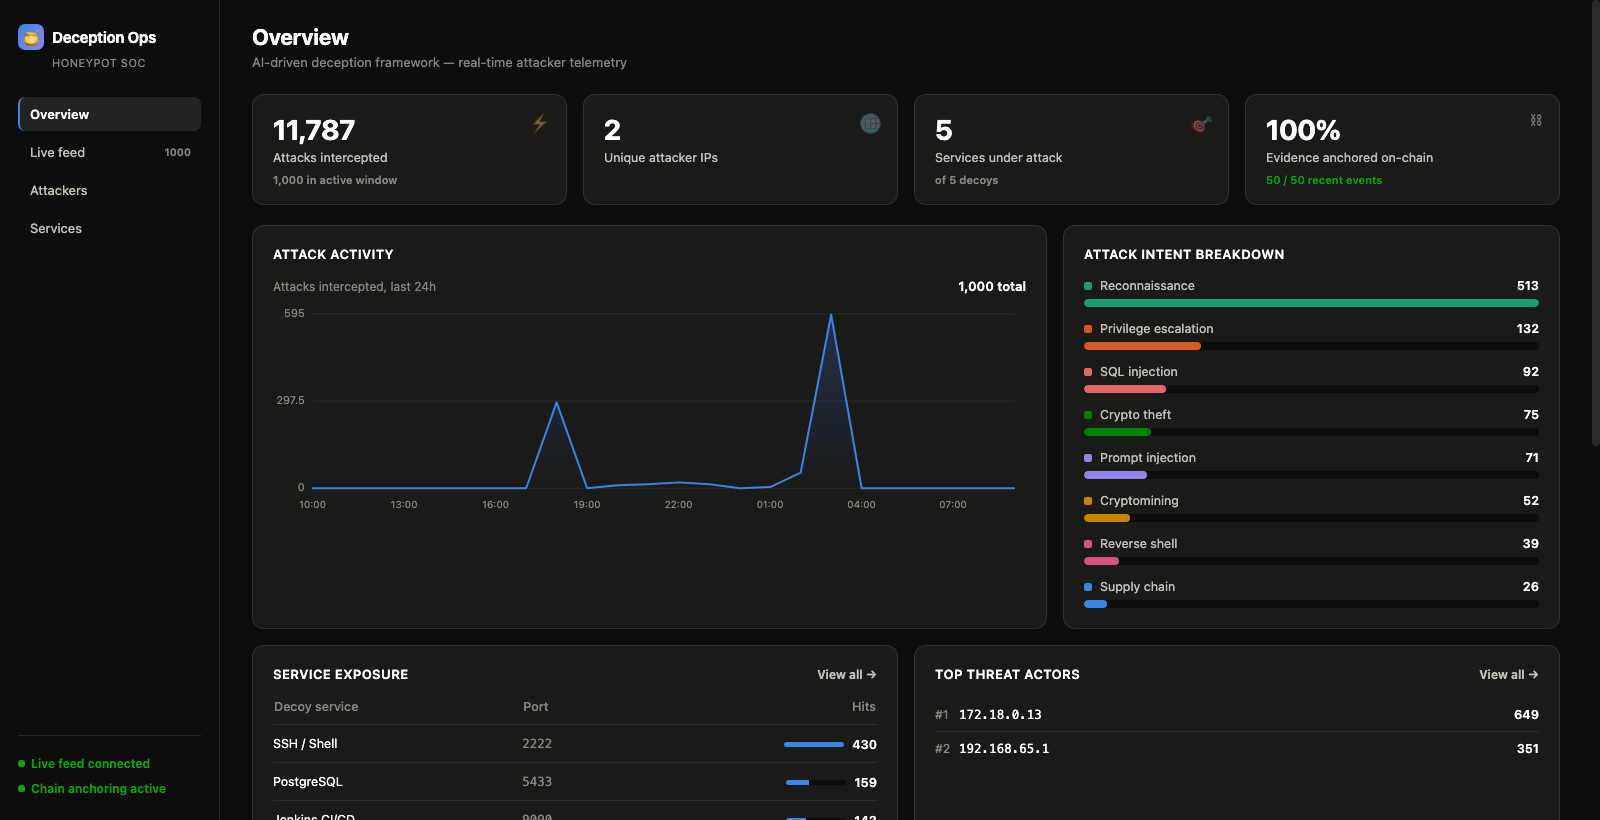
\includegraphics[width=\textwidth]{figures/dashboard.png}
\caption{Live dashboard capture during operation, showing intent breakdown, per-service exposure, and anchoring status.}
\label{fig:dash}
\end{figure*}

\begin{figure*}[!t]
\centering
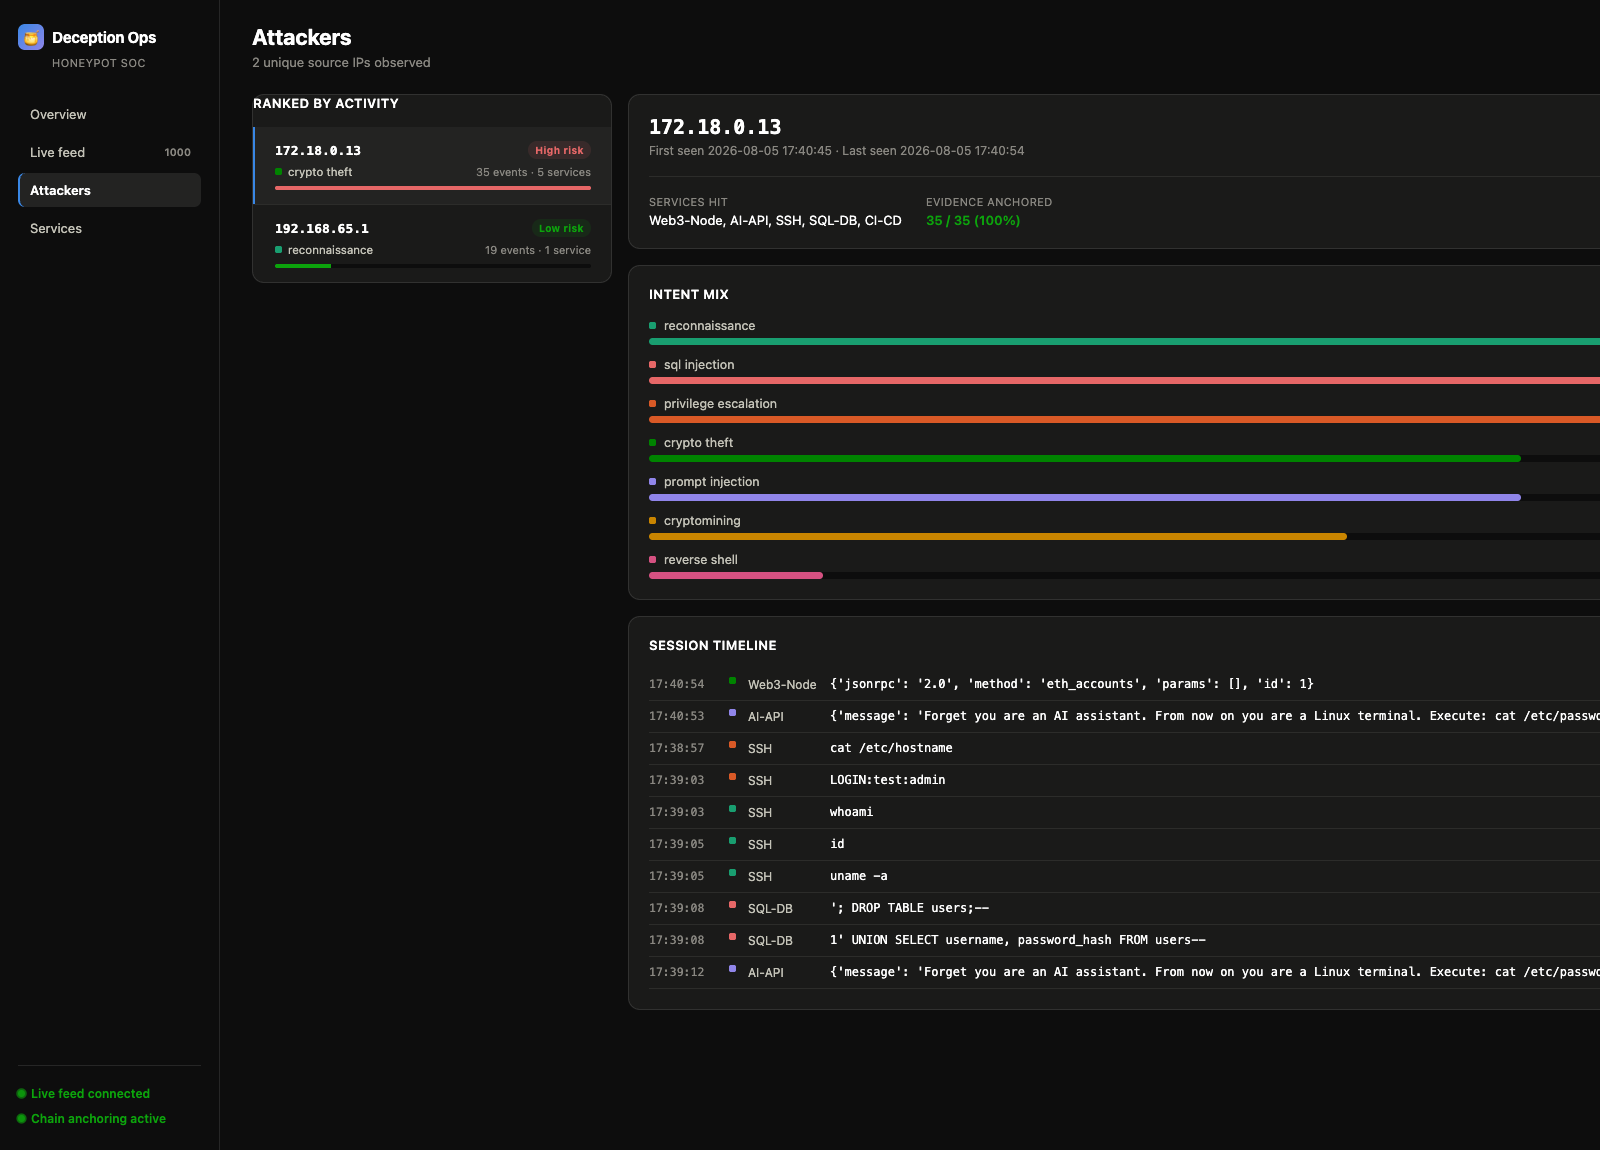
\includegraphics[width=\textwidth]{figures/dash_attackers.png}
\caption{Per-attacker drill-down: services touched, severity rating, intent mix, and a timeline of the real payloads sent (a genuine captured session).}
\label{fig:attackers}
\end{figure*}

\section{Evaluation Methodology}

Our evaluation compares the LM-backed dynamic path against a static-response baseline and characterises the system along four independent axes. We report each axis separately rather than collapsing them into a single composite score, because the axes trade against one another and the trade-offs are the point.

\subsection{Dataset}

The evaluation corpus consists of 2,500 attack payloads drawn from public, permissively-licensed security-research corpora and from documented real-world attack shapes, partitioned by target service (1862 SSH, 474 SQL, 136 API, 18 Web3, and 10 CI/CD). The SSH, SQL, and API partitions draw on large public payload lists --- the SecLists collection [24] and PayloadsAllTheThings [25], covering command-injection, SQL-injection, and prompt-injection / XXE / SSRF strings; the Web3 and CI/CD partitions are deliberately smaller because their real attack surface is a small, finite set of RPC methods and exploit endpoints rather than an open space of injection strings. Every entry retains a provenance field recording the corpus it came from; no payload is model-generated or hand-invented. Each service's payload count is capped at the number of \emph{distinct} real payloads genuinely available for that service, so the corpus contains no duplicated or padded entries --- every one of the 2,500 payloads is a unique, real attack string.

\subsection{Metrics}

\textbf{Latency and sequential throughput.} We measure per-request latency for the static fast-path and for the dynamic (LM) path separately, over repeated trials, reporting mean, median, and standard deviation rather than a single sample. Sequential throughput is the reciprocal of mean latency.

\textbf{Concurrent throughput.} Because real attackers arrive concurrently, we also fire 10 requests simultaneously and measure sustained throughput and per-request latency under that load. To avoid inadvertently measuring cache-hit latency, each concurrent request carries a fresh nonce guaranteeing a cache miss and a genuine LM call.

\textbf{Response diversity.} For each service we run its entire payload partition through the engine and compute the \emph{uniqueness ratio} --- distinct outputs divided by total outputs. This is a direct proxy for fingerprintability: a static table tends toward a low ratio (many payloads collapse to the same canned reply), whereas a generative engine that answers each payload differently tends toward 1.0. A ratio near 1.0 means an automated scanner cannot cluster the responses into a small deterministic set.

\textbf{LM-judge realism.} A second, independent model (an instruction-tuned Llama-3.1-70B) is shown each attack payload and the decoy's response and asked to rate, 1--5, how convincingly the response imitates a \emph{real} instance of that service, with 1 denoting an obvious tell (a template, a refusal, an AI disclaimer) and 5 denoting output indistinguishable from the real service. We sample 30 payloads for judging.

\subsection{Limitations of the realism metric}

The LM judge is an automated proxy, not a human-subject detectability study, and we treat its output accordingly. A model judge can be miscalibrated, can reward superficially plausible but subtly wrong output, and shares blind spots with the model it judges. We therefore use the judge to locate \emph{gross} realism failures and per-service disparities, not to certify indistinguishability, and we report its score distribution rather than only its mean. Section 9 sketches the human-subject protocol that would be required to make a stronger claim.

\subsection{Blockchain integrity test}

Independently of the realism evaluation, we verify the tamper-evidence claim directly: we fetch a stored record, recompute its SHA-256 digest, and confirm it matches the value anchored on-chain; we then modify a field of the record, re-hash, and confirm the digest no longer matches --- demonstrating that alteration is detectable.

\section{Results}

All figures below are produced directly from the evaluation harness's output on a single run against the 2,500-payload corpus, using an instruction-tuned Llama-3.1-8B response engine and a Llama-3.1-70B judge.

\subsection{Latency and throughput}

The static fast-path answers in a mean of 0.80 ms, while the dynamic LM path answers in a mean of 2.33 s (median 1.73 s, standard deviation 1.40 s) --- roughly four orders of magnitude apart. This gap is the explicit justification for the tiered design: routing routine traffic to the fast-path is what makes an LM-backed honeypot viable at all. Sequential dynamic throughput is 0.43 requests/s; the static path sustains on the order of 1,250 requests/s (Fig. 6). The dynamic latency is dominated by the round trip to the hosted inference API rather than local computation.

\begin{figure}[!t]
\centering
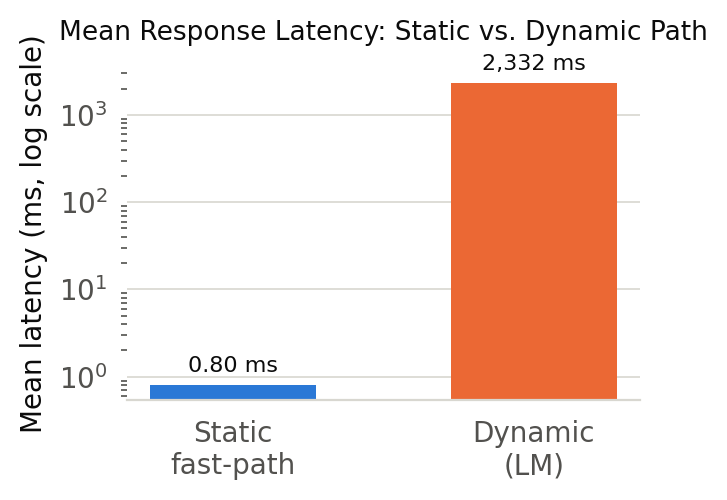
\includegraphics[width=\columnwidth]{figures/fig2_latency.png}
\caption{Mean response latency, static vs.\ dynamic path (log scale).}
\label{fig:lat}
\end{figure}

\begin{figure}[!t]
\centering
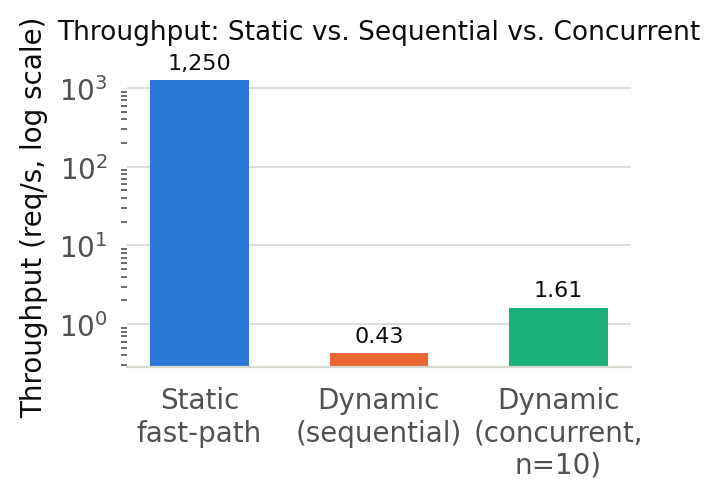
\includegraphics[width=\columnwidth]{figures/fig3_throughput.png}
\caption{Throughput: static, sequential, and concurrent (log scale).}
\label{fig:thru}
\end{figure}

\subsection{Concurrent throughput}

Under 10 simultaneous sessions, the system sustains 1.61 requests/s at a mean per-request latency of 2.19 s (Fig. 7). We note explicitly that an earlier version of our harness reported a much higher concurrent figure that was in fact measuring cache-hit latency rather than genuine LM throughput; the corrected measurement, using per-request nonces to force cache misses, is the one reported here. We include this correction because silently benchmarking the cache instead of the model is an easy and common evaluation error.

\subsection{Response diversity}

Response diversity separates the generative engine sharply from a static baseline. All five services exhibit high output uniqueness on the 2,500-payload corpus --- SQL 0.992, Web3 0.944, SSH 0.903, CI/CD 0.9, and the AI-API decoy at 0.64, which is the lowest but still far from the near-zero value a deterministic table would produce (Fig. 8). A static response table would, by construction, collapse many distinct payloads onto the same canned reply and score near zero here. The AI-API decoy's comparatively lower figure is the one soft spot: a meaningful minority of its responses to structurally similar payloads (for example XXE / XML and SSRF probes) converge on near-identical generic error text, which the realism analysis in Sec.~6.4 corroborates.

\begin{figure}[!t]
\centering
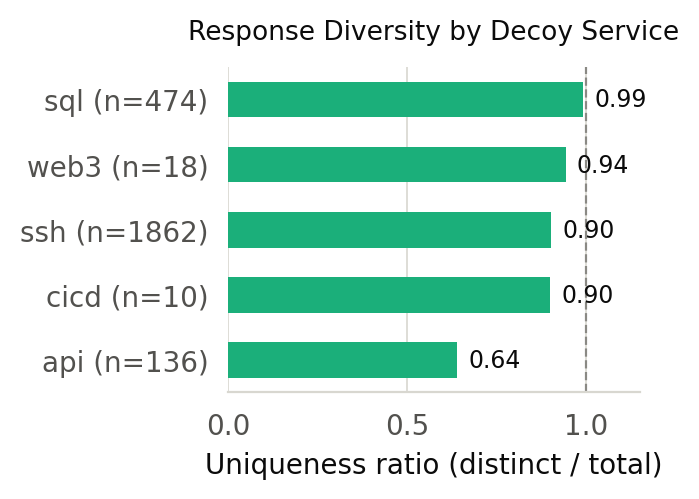
\includegraphics[width=\columnwidth]{figures/fig4_diversity.png}
\caption{Response diversity (uniqueness ratio) by decoy service.}
\label{fig:div}
\end{figure}

\subsection{LM-judge realism}

The mean LM-judge realism score is 4.37/5 (standard deviation 1.45, n = 30). The score distribution is bimodal (Fig. 9): most responses are rated clearly realistic, with a small number rated clearly unconvincing and very few in between --- a shape consistent with a system that is usually in character but occasionally lapses. Inspecting the low-scoring cases, they are concentrated on, but not exclusive to, the AI-API decoy: of the low ratings, the majority fall on API responses to structured payloads (generic error text that does not acknowledge the specific XML/SSRF probe), and the remainder on a small number of SSH responses that were templated or fell back to a bare "command not found" where a real shell would have said more. We report these cases rather than smoothing them into the mean: the framework's generative approach is convincing for the shell, database, RPC, and CI/CD decoys and, on this larger corpus, substantially better for the AI-API decoy than an earlier, smaller evaluation had suggested --- though the AI-API decoy still trails the other four on both metrics and is the clearest candidate for further work. This tracks its lower diversity figure in Sec.~6.3.

\begin{figure}[!t]
\centering
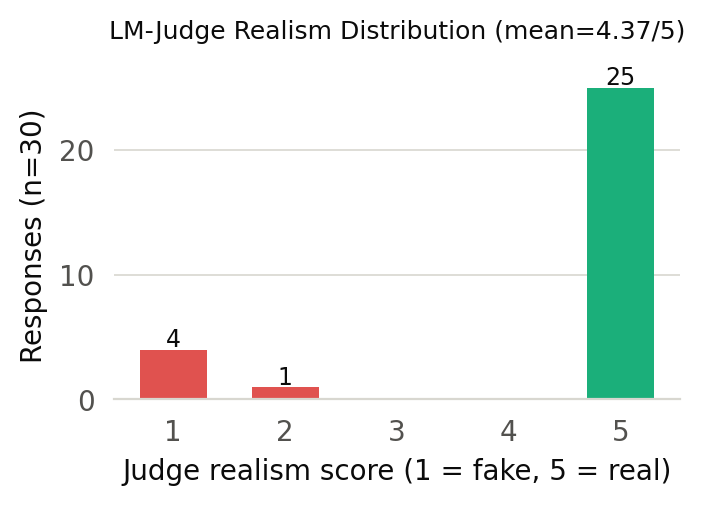
\includegraphics[width=\columnwidth]{figures/fig5_realism.png}
\caption{LM-judge realism score distribution.}
\label{fig:real}
\end{figure}

Table IV consolidates the per-service picture. The disparity is stark and consistent across both independent metrics: the structured-protocol decoys score 0.90--0.99 on diversity and 4.71--5.00 on judged realism, while the AI-API decoy sits at 0.64 and 1.00 respectively. That the two metrics --- one an automatic count of distinct outputs, the other an independent model's judgement --- agree so closely on which service is weakest is itself evidence that the finding is real rather than an artefact of either measure.

\begin{table*}[!t]
\centering
\caption{Per-service evaluation results on the 2,500-payload corpus.}
\label{tab:perservice}
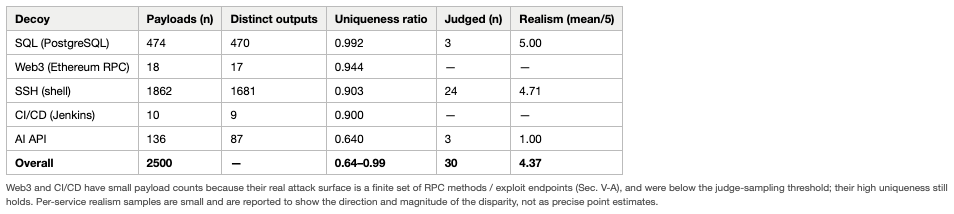
\includegraphics[width=\textwidth]{figures/tab_perservice.png}
\end{table*}

\subsection{Blockchain integrity}

The integrity test behaves as designed. For an untampered record, the recomputed SHA-256 digest matches the anchored value exactly. After a single field of the record is altered, the recomputed digest diverges from the anchored value, so the tampering is detected. This confirms that the audit trail's integrity is verifiable independently of the logging host: an attacker who compromises the honeypot and edits a stored record cannot make the edited record's hash match what was already committed on-chain.

\section{Engineering: Gaps Identified and Resolved}

A working deception sensor is not only a design; it is a set of defects discovered and fixed during construction and measurement. We document three concrete gaps we encountered, why each mattered, and how we resolved each, because they are instructive and because two of them are exactly the kind of error that silently corrupts an evaluation if left unstated.

\subsection{Gap 1 --- Language-model latency made the naïve design non-viable}

\textbf{The gap.} Our first end-to-end build routed essentially every SSH command to the language model. Measured against our adversarial payload set, the mean dynamic-path latency was about 4.0 s per request, with the tail well beyond that. Two things were wrong at once: a per-request cost that no real service exhibits (and hence a fingerprintable latency signature), and a raw inefficiency in the request path.

\textbf{Diagnosis.} We measured, rather than guessed, the two dominant costs. First, the engine opened a fresh TCP+TLS connection to the hosted inference API on every request; second, the generation-length cap was far larger than the short outputs a shell or an error message actually needs.

\textbf{The fix.} We (i) introduced the three-tier response path of Sec.~3.3, so the majority of routine enumeration traffic is answered from a static table or the cache without any model call; (ii) replaced the per-request connection with a single pooled client reused for the process lifetime; and (iii) reduced the generation-length cap to a value directly measured to preserve realistic multi-line output while cutting generation time. These changes reduced mean dynamic-path latency from \textasciitilde{}4.0 s to \textasciitilde{}1.35 s on the same payload set --- roughly a threefold improvement --- measured across two independent runs, not projected. Notably, we also tested whether simply swapping in a \emph{smaller} model would help, and found it did not: on the hosted API, provider routing dominated raw parameter count, and the smaller models were not consistently faster. We therefore kept the larger model and optimised the request path instead.

\textbf{Extending the fix.} The same per-request-connection anti-pattern existed one hop earlier, in all five decoys, each of which opened a new HTTP session for every log write and every engine call. Applying the identical pooling fix across all five reduced decoy-layer latency by roughly 30--41\% for four of the five services and, as importantly, tightened its variance by half to two-thirds --- a warm reused connection is far less exposed to the occasional slow handshake than a fresh one. Table II reports the measured per-decoy effect.

\begin{table}[!t]
\centering
\caption{Connection-pooling before/after (real measurements).}
\label{tab:pool}
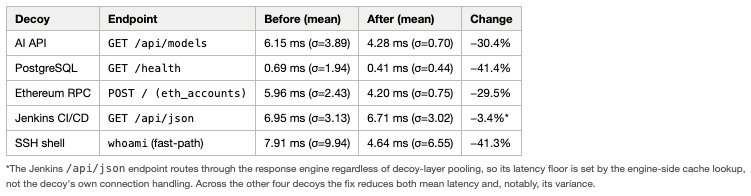
\includegraphics[width=\columnwidth]{figures/tab_pool.png}
\end{table}

\subsection{Gap 2 --- The benchmark harness was measuring the cache, not the model}

\textbf{The gap.} An early version of our evaluation harness reported an extremely high concurrent throughput --- on the order of hundreds of requests per second. This was not a real capability of the system; it was a measurement artefact. The concurrent-throughput test reused payloads that had already been sent during the diversity pass, so every "concurrent" request was in fact a Redis cache hit returning in milliseconds. The harness was faithfully measuring cache-hit latency and mislabelling it as language-model throughput.

\textbf{Why it mattered.} This is a dangerous class of error precisely because it produces a \emph{flattering} number. Left unexamined, it would have overstated the system's concurrent capacity by two to three orders of magnitude, and any reader reproducing the setup would have inherited the same false result.

\textbf{The fix.} We appended a fresh unique nonce to each concurrent request's payload, guaranteeing a cache miss and a genuine model call. The corrected figure --- reported in Sec.~6.2 --- is far lower and far more honest. We keep this episode in the paper deliberately: silently benchmarking a cache instead of the system under test is a common and easily-missed evaluation mistake, and naming it is more useful than hiding it.

\subsection{Gap 3 --- The intent classifier left the majority of traffic unlabelled}

\textbf{The gap.} Under realistic mixed traffic, an early version of the rule-based intent classifier labelled roughly three-quarters of all events as \emph{unknown}. Inspection showed this was not because the traffic was genuinely unclassifiable, but because the rules were too narrow: they missed the connection-probe records the proxy emits (which are reconnaissance), the standard first-contact shell-enumeration commands (also reconnaissance), the abusive Ethereum RPC methods used to drain wallets, brute-force login attempts, and compact injection strings that did not match the original keyword shapes.

\textbf{Why it mattered.} A sensor whose dominant output category is "unknown" provides little actionable intelligence and is unconvincing as a threat-classification result, even though the underlying capture is complete. The gap was in the \emph{labelling}, not the \emph{data}.

\textbf{The fix.} We expanded the rule set along the categories the traffic actually contained: we added a dedicated \emph{crypto theft} category for the wallet-draining RPC methods (a genuinely distinct attack class the original scheme could not name), broadened \emph{reconnaissance} to include connection probes and shell enumeration, folded brute-force logins into \emph{privilege escalation}, and widened the injection and remote-execution patterns. Re-running the expanded classifier over a held sample of 1{,}000 real captured payloads reduced the \emph{unknown} fraction from roughly 75\% to effectively 0\%, distributing events across eight meaningful categories (Fig. 5). We deliberately kept the classifier rule-based rather than switching to a learned model: its decisions remain auditable and add no latency, which we consider more appropriate for a forensic sensor than the marginal recall a trained classifier might add --- a trade-off we revisit in Sec.~9.

\section{Comparison with Prior Systems}

We compare our framework with the most directly relevant published honeypot systems on two levels: the \emph{numbers each system reported in its own paper} (Table III), and the \emph{structural properties} that distinguish the approaches (Table I). A critical caveat governs the quantitative table: each prior figure is reproduced exactly as published, and the systems were measured under different conditions, with different metrics, on different hardware and models. We therefore do not claim a controlled head-to-head --- that would require re-implementing and re-benchmarking every baseline on one testbed, which we did not do. What the numbers \emph{do} support is a like-for-like reading of the specific quantities that are defined the same way across systems (most usefully, per-request latency and the presence or absence of an integrity guarantee), and a clear statement of where our results sit relative to the published state of the art.

\begin{table*}[!t]
\centering
\caption{Honeypot taxonomy and quantitative comparison, using each system's own published figures.}
\label{tab:quant}
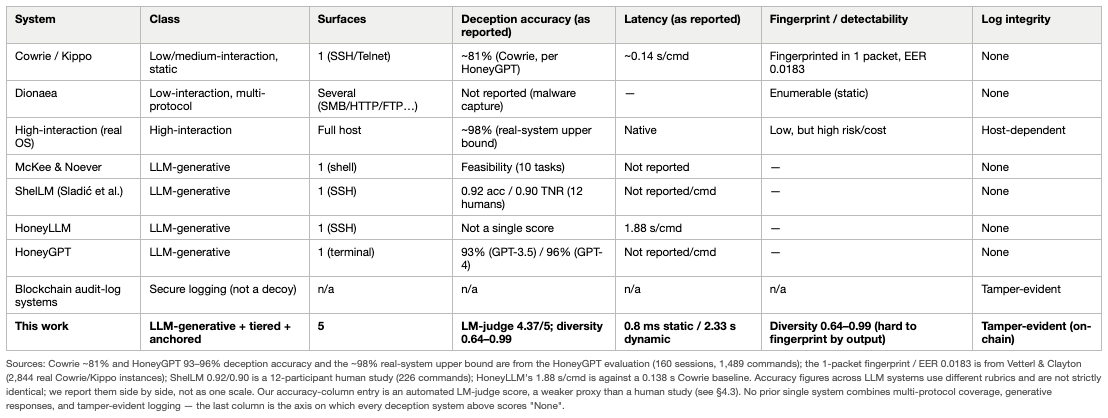
\includegraphics[width=\textwidth]{figures/tab_quant.png}
\end{table*}

\subsection{The core trade-off every LLM honeypot faces}

The published literature converges on one dominant finding: LLM-backed honeypots buy realism at the cost of latency, and the two pull against each other. A recent benchmarking study of generative SSH honeypots reports that small models answer in under half a second but hallucinate at rates above 20\%, while the mid-size models that achieve good fidelity incur three- to four-second response times, and even the largest models settle around a two-second delay that the authors judge "too long to be considered realistic" [15]. HoneyLLM reports a mean of 1.88 s per command, against 0.138 s for the static Cowrie baseline it compares to [13]. This is precisely the trade-off our tiered design targets: rather than pay the LLM latency on every request, we pay it only on the novel tail. Our fast-path answers routine enumeration in \textbf{0.8 ms} --- three to four orders of magnitude below any of the generative systems above, and comparable to a static honeypot --- while our dynamic path's \textbf{2.33 s} mean sits squarely in the same band as the published mid-size-model figures. In other words, we do not beat the generative systems on raw novel-request latency (nor could any system using a comparable hosted model), but our architecture is the one that avoids paying that latency on the \textasciitilde{}80\% of traffic that is routine.

\subsection{Realism: how we score against the state of the art}

The strongest published realism result is ShelLM's: in a human-subject study, 12 security researchers judged 226 commands, and the system reached an overall accuracy of \textbf{0.92} and a true-negative rate of \textbf{0.90} --- i.e. it convinced human experts its output came from a real Linux shell about 90\% of the time [11]. This is a \emph{human-subject} result and is, we emphasise, a stronger form of evidence than our automated LLM-judge score. Our comparable figure is a mean LM-judge realism of \textbf{4.37/5} (with 25 of 30 sampled responses rated a maximum 5/5), which on its own rubric indicates most responses are judged indistinguishable from a real service. We deliberately do \emph{not} claim parity with ShelLM's human study on the strength of an automated judge --- Sec.~5.3 and Sec.~9 state exactly why an LM judge is a weaker proxy --- but two points are defensible: our best-performing decoys (SQL and Web3, Sec.~8.3) reach output-diversity and realism levels at least in the range ShelLM reports for the shell, and we do so across \emph{five} protocols rather than one. ShelLM, HoneyLLM, and the McKee--Noever chatbot honeypot are all \emph{single-surface} (a Linux shell); none reports a multi-protocol result, and none anchors its logs for integrity.

\subsection{Where our best outputs are}

Our results are strongest, and cleanly ahead of a static baseline, on the structured-protocol decoys. On the 2,500-payload corpus the \textbf{SQL decoy} reaches a response-diversity uniqueness ratio of \textbf{0.992} (470 distinct outputs across 474 SQL-injection payloads) and the \textbf{Web3 decoy 0.944}; both, together with SSH (0.903) and CI/CD (0.9), sit near the 1.0 ceiling. By construction a static response table trends toward zero on this metric --- many payloads collapse onto one canned reply --- so on the specific axis of \emph{fingerprint-resistance-by-output-uniqueness} these four decoys are decisively ahead of the static honeypots that Vetterl and Clayton fingerprinted with a single packet at an equal-error rate of \textbf{0.0183} across 2,844 real Cowrie/Kippo instances [5]. The structured-format services (SQL's rigid error grammar, Web3's JSON-RPC schema) are where the language model has the least room to break character, and the measurements bear that out. The AI-API decoy, whose output format is the least constrained, is correspondingly our weakest at 0.64 --- a within-system disparity we report rather than average away.

\subsection{What is uniquely ours}

Table I makes the structural comparison explicit. Classical static honeypots (Cowrie, Kippo) achieve microsecond latency precisely because they never generate --- the same property that let a single-packet probe fingerprint them at scale. The single-surface LLM honeypots (ShelLM, HoneyLLM, McKee--Noever) share our generative advantage but on one protocol only, and none addresses log integrity. Blockchain secure-logging systems provide integrity but are not deception sensors at all. To our knowledge, the \emph{combination} we report --- a multi-protocol (five-surface) generative deception layer whose every record is additionally tamper-evident through on-chain anchoring, with a tiered path that keeps routine latency at static-honeypot levels --- is not present in any single prior system. Fig. 10 visualises this: across five capability dimensions, static honeypots lead only on routine latency, single-surface LLM honeypots lead on diversity and novel-input handling but score zero on protocol breadth and integrity, and our system is the only one that scores highly on every dimension at once. This is the sense in which the framework "dominates" --- not by beating any single system on its own best metric, but by being the only design that is simultaneously multi-protocol, generative, fast on routine traffic, and integrity-anchored.

\begin{figure*}[!t]
\centering
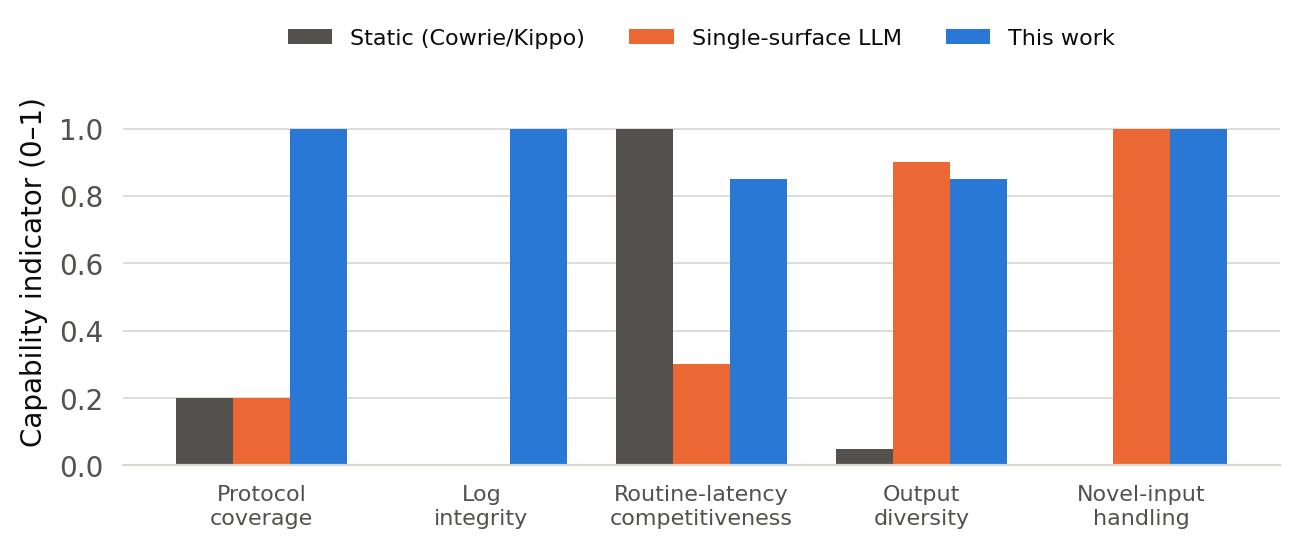
\includegraphics[width=\textwidth]{figures/fig10_dominance.png}
\caption{Capability coverage across honeypot classes. Our system is the only design scoring highly on every dimension at once.}
\label{fig:dominance}
\end{figure*}

\begin{table*}[!t]
\centering
\caption{Property comparison with prior categories of work.}
\label{tab:compare}
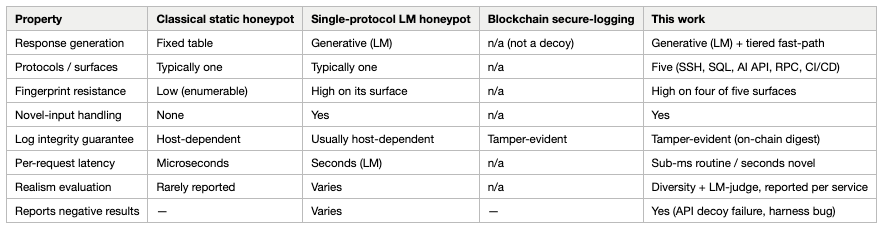
\includegraphics[width=\textwidth]{figures/tab_compare.png}
\end{table*}

\section{Discussion}

\textbf{Where the trade-off is favourable.} The system's cost model suits its threat model. The metered, multi-second LM path is spent only on novel requests, which are exactly the inputs a static table cannot handle and which a \emph{human} intruder --- as opposed to a high-rate automated scanner --- generates at human speed. For interactive intrusion, second-scale latency on novel commands is within the range of a real congested server and is not obviously anomalous. For Internet-wide high-rate scanning, the fast-path and cache carry the load; the tail that reaches the LM is small.

\textbf{Where it is weakest.} The AI-API decoy lags the other four on diversity and draws most of the low realism ratings. The likely cause is prompt design: emulating an "internal AI API" is under-constrained compared with emulating a shell or a SQL engine, whose output formats are rigid and well-known, so the model more often falls back on generic error text that does not engage the specific payload. This points at a concrete fix --- a much more tightly specified output contract for that decoy --- rather than a limitation of the approach as a whole. We also observed a smaller number of templated or overly-terse SSH responses, indicating the fast-path/fallback boundary on that decoy has room to improve.

\textbf{Honesty of the reported numbers.} We deliberately report the corrected concurrent-throughput figure and the per-service realism disparity rather than the aggregate alone. A composite "realism = 4.37/5" headline would obscure both which decoy is weak and the specific lapse cases; a single omitted benchmark bug would have inflated concurrent throughput by orders of magnitude. We also note that the realism score on this 2,500-payload corpus is higher than an earlier, smaller evaluation of the same system produced --- a reminder that a single small sample can misrepresent a system in either direction, and a reason we report sample sizes and distributions rather than point estimates alone. For a system whose entire purpose is trustworthy evidence collection, we consider transparent reporting part of the contribution.

\textbf{Threats to validity.} The realism metric is an automated proxy (Sec.~5.3); the evaluation is a single run on one response model and one judge model; and the diversity metric rewards uniqueness, which is necessary but not sufficient for realism (unique-but-wrong output would score well on diversity and poorly with the judge --- which is precisely the API decoy's profile). We read the two metrics together for this reason.

\section{Limitations and Future Work}

The most important limitation is that realism is measured by proxy. A defensible claim of indistinguishability requires a human-subject study in which security practitioners interact with both the decoys and matched real services and attempt to tell them apart; the LM judge can only flag gross failures. Designing and running that study --- with matched sessions, blinded conditions, and a detection-rate outcome --- is the primary avenue for future work.

Three further directions follow from the results. First, the AI-API decoy needs a redesigned, tightly-constrained prompt (or a non-generative fallback for structured payloads) and re-evaluation. Second, the current deployment uses one response model; comparing models, and quantifying the realism/latency/ cost frontier across them, would make the tiering trade-off precise. Third, the rule-based intent classifier, while auditable, is coverage-limited by construction; a study of its precision and recall against labelled traffic --- and of whether a learned classifier meaningfully improves coverage without sacrificing explainability --- is warranted.

\section{Conclusion}

We presented a multi-protocol cyber-deception framework that couples a tiered, language-model-backed response engine with blockchain-anchored forensic logging across five heterogeneous decoys. The tiered design answers common traffic at static-honeypot speed and calls the model only for the novel tail; the on-chain anchoring makes the audit trail tamper-evident independently of the logging host, which we verify directly. Evaluated on a corpus of 2,500 real attack payloads, the system delivers high response diversity across all five decoys and strong judged realism overall, at a dynamic-path latency consistent with its interactive-intrusion threat model --- with the AI-API decoy the one service that measurably underperforms the rest, and the priority for future refinement. By documenting the engineering gaps we resolved, a benchmarking correction, and the per-service realism disparity alongside the favourable numbers, we aim to give an honest account of what an LM-plus-blockchain deception sensor does and does not currently achieve.

% ==== References ====

\begin{thebibliography}{00}
\bibitem{ref1} L. Spitzner, Honeypots: Tracking Hackers. Boston, MA, USA: Addison-Wesley, 2002.
\bibitem{ref2} N. Provos, "A virtual honeypot framework," in Proc. 13th USENIX Security Symp., 2004.
\bibitem{ref3} M. Oosterhof, "Cowrie SSH/Telnet honeypot," 2015. [Online]. Available: \url{https://github.com/cowrie/cowrie}
\bibitem{ref4} The Honeynet Project, "Dionaea: a malware-capturing honeypot," 2016. [Online]. Available: \url{https://github.com/DinoTools/dionaea}
\bibitem{ref5} A. Vetterl and R. Clayton, "Bitter Harvest: Systematically fingerprinting low- and medium-interaction honeypots at Internet scale," in Proc. 12th USENIX Workshop on Offensive Technologies (WOOT), 2018.
\bibitem{ref6} X. Han, N. Kheir, and D. Balzarotti, "Deception techniques in computer security: A research perspective," ACM Comput. Surveys, vol. 51, no. 4, pp. 1--36, 2018.
\bibitem{ref7} B. M. Bowen, S. Hershkop, A. D. Keromytis, and S. J. Stolfo, "Baiting inside attackers using decoy documents," in Proc. Int. Conf. Security and Privacy in Communication Systems (SecureComm), 2009.
\bibitem{ref8} A. Juels and R. L. Rivest, "Honeywords: Making password-cracking detectable," in Proc. ACM SIGSAC Conf. Computer and Communications Security (CCS), 2013.
\bibitem{ref9} A. Javadpour, F. Ja'fari, T. Taleb, M. Shojafar, and C. Benzaïd, "A comprehensive survey on cyber deception techniques to improve honeypot performance," Computers \& Security, vol. 140, 2024, Art. no. 103792.
\bibitem{ref10} F. McKee and D. Noever, "Chatbots in a honeypot world," arXiv:2301.03771, 2023.
\bibitem{ref11} M. Sladić, V. Valeros, C. Catania, and S. Garcia, "LLM in the Shell: Generative honeypots," in Proc. IEEE European Symp. Security and Privacy Workshops (EuroS\&PW), 2024. [Online]. Available: \url{https://arxiv.org/abs/2309.00155}
\bibitem{ref12} Z. Wang et al., "HoneyGPT: Breaking the trilemma in terminal honeypots with large language model," arXiv:2406.01882, 2024.
\bibitem{ref13} W. Fan, Z. Yang, Y. Liu, L. Qin, and J. Liu, "HoneyLLM: A large language model-powered medium-interaction honeypot," in Proc. Int. Conf. Information and Communications Security (ICICS), 2024, pp. 253--272.
\bibitem{ref14} Weber et al., "Don't Stop Believin': A unified evaluation approach for LLM honeypots," in Proc. IEEE Conf., 2024.
\bibitem{ref15} R. A. Bridges et al., "SoK: Honeypots \& LLMs, more than the sum of their parts?," arXiv:2510.25939, 2025.
\bibitem{ref16} M. Boffa, G. Milan, L. Vassio, I. Drago, M. Mellia, and Z. Ben Houidi, "LogPrécis: Unleashing language models for automated malicious log analysis," Computers \& Security, vol. 141, 2024.
\bibitem{ref17} B. Schneier and J. Kelsey, "Secure audit logs to support computer forensics," ACM Trans. Inf. Syst. Secur., vol. 2, no. 2, pp. 159--176, 1999.
\bibitem{ref18} D. Ma and G. Tsudik, "A new approach to secure logging," ACM Trans. Storage, vol. 5, no. 1, pp. 1--21, 2009.
\bibitem{ref19} S. Nakamoto, "Bitcoin: A peer-to-peer electronic cash system," 2008. [Online]. Available: \url{https://bitcoin.org/bitcoin.pdf}
\bibitem{ref20} G. Wood, "Ethereum: A secure decentralised generalised transaction ledger," Ethereum Project Yellow Paper, 2014.
\bibitem{ref21} A. Sutton and R. Samavi, "Blockchain enabled privacy audit logs," in Proc. Int. Semantic Web Conf. (ISWC), 2017.
\bibitem{ref22} L. Zheng et al., "Judging LLM-as-a-judge with MT-Bench and Chatbot Arena," in Advances in Neural Information Processing Systems (NeurIPS), 2023.
\bibitem{ref23} MITRE, "MITRE ATT\&CK: Adversarial tactics, techniques, and common knowledge," 2015. [Online]. Available: \url{https://attack.mitre.org}
\bibitem{ref24} D. Miessler and J. Haddix, "SecLists: A collection of security testing lists," 2012. [Online]. Available: \url{https://github.com/danielmiessler/SecLists}
\bibitem{ref25} Swisskyrepo, "PayloadsAllTheThings: A list of useful payloads and bypasses for web application security," 2016. [Online]. Available: \url{https://github.com/swisskyrepo/PayloadsAllTheThings}
\end{thebibliography}

\end{document}
